\chapter{Design}

\section{Providers}
A testing framework that aims to validate an entire distribution has far reaching requirements and should be capable to test mostly any software system while not hindering the testing process. To make it more probable that Ellida will be able to cover any aspect of a specification a model based on test providers was developed.

A \textbf{provider} is defined as a testing framework, tool or collection of tests focused on a specific subsystem or providing a specialised functionality. The providers are supported through classes that expose a uniform interface but abstract away the details such as executing specific files and parsing logs. Examples of providers are the LTP test suite, Image Tests - Yocto specific functionality that allows Python based unit tests to run through ssh, Lynis security auditing tool, Phoronix benchmarking platform, and LTTng tracing framework.

Specifications can be formally viewed as a set of categorized requirements as discussed in the abstraction section (\ref{specs}). Every category of requirements is usually specific to a particular subsystem or abstract attribute that the target system should have. Even if the abstract requirements are defined as categories and then split into more concrete, technical requirements, they still tend to be fairly vague, or leave room for interpretation.

The model proposed in the Ellida framework represents every such small technical requirement as a list of test sets, every set having a unique provider. A single requirement can therefore be tested with each and every provider while keeping the tests separated and organised on sets. A set can contain one or multiple tests, but requires that all tests are specific to the same provider. For example, the AGL.711 requirement can be validated by a list of two sets - A and B - with set A using the Core as provider and set B using LTP. The A set will contain one or more Python scripts while the B set will use LTP control files.

\begin{figure}[h!]
  \centering
	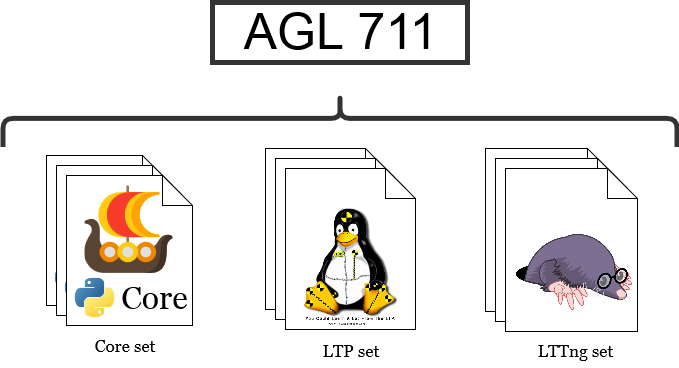
\includegraphics[width=0.6\textwidth]{images/providers.png}
    \caption{Validation based on multiple providers}
\end{figure}

\section{Specification abstraction and the test suite} \label{specs}
The specification representation is one of the important design features within the framework. The format has to be extensible, easy to use by both users and developers, with little or no constrains. The specifications consist of a folder tree structure that follows the underlying model of both AGL and CGL. The tree is populated with JSON files containing metadata relevant to each requirement.

Mirroring a specifications structure, a test suite uses the same format but further develops it to contain test files. Instead of having requirements as tree leafs, each requirement is a folder containing one or more sets. A set is just another folder with a provider specific structure whose only requirement is to contain a JSON document describing the set.

 
\begin{figure}[htb!]
	\begin{minipage}{0.48\textwidth} \centering
	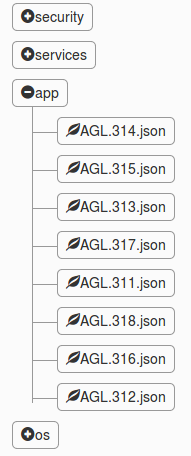
\includegraphics[width=0.5\linewidth]{images/agl_spec.png}
	\caption{AGL representation}
    \end{minipage} \hfill
    \begin{minipage}{0.48\textwidth} \centering
	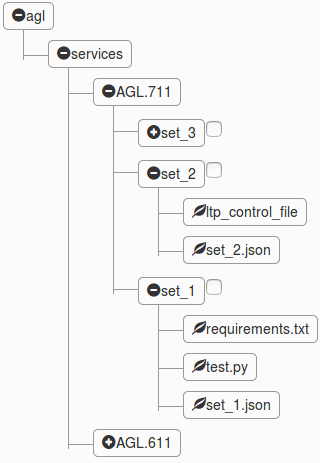
\includegraphics[width=0.82\linewidth]{images/test_suite.png}
	\caption{Test suite example}
    \end{minipage}
\end{figure}


\section{Architecture}
Ellida framework consists of two main parts - the actual application that provides all the functionality and metadata files. The metadata is organised as an OpenEmbedded layer and is used for integration with Poky. The framework is made up of several components that communicate through sockets and TCP connections. They can run on different machines and different networks as long as the settings are properly configured and the connections can be created. The main components are the \textbf{Engine}, the \textbf{Manager}, the \textbf{Controller} and the \textbf{Daemon}. They are loosely coupled to allow for as much flexibility as possible and enable scaling of the testing process.

In terms of communication and UI, relatively new but mature technologies were used such as ZeroMQ, WebSockets and Flask. The functional part of the framework is written only in Python, while the setup part uses Bitbake specific syntax that allows for a combination of Shell script and Python.

The \textbf{Engine} is at the centre of the communication system. Almost all communication has to pass through the Engine with no two components directly communicating with each other. The reason behind this design choice is that a centralized system is much easier to implement, monitor and control than a system where each component can communicate with every other component. It also enables a more predictable and manageable scaling process. Considering that Engines main task is to manage communication, the impact on overall efficiency is low enough not to outweigh the benefits. The \textbf{Manager} is responsible with the specification representation and keeps the test suite organized. The \textbf{Controller} is a user interface - the main I/O system and the \textbf{Daemon} is the part of the framework that runs on target distributions and executes the tests.

\subsection{Technologies}
\subsubsection*{ZeroMQ}
The backbone of the communication system is the ZeroMQ (ZMQ) library. It provides very efficient, highly scalable means of communication that abstracts most of the laborious setup usually required by network based systems. ZMQ is able to carry messages across inproc, IPC, TCP, TIPC, multicast and provides patterns recurrent in distributed systems such as push-pull and router-dealer. The testing framework uses a more common pattern - socket pair, and TCP connections. The Engine uses ZMQ polling to listen for multiple connections coming from different components.

\subsubsection*{Flask}
The Controller component is a web application with a Flask based backend. Flask is a Python web framework that is lightweight, very configurable and easy to setup. It is considered to be a microframework as it comes with only a couple of dependencies and only one development restriction - that the application project has a predefined structure. Its simplicity makes it an excellent choice for an application that needs to be as extensible as possible. The code base as well as the necessary setup are reduced, while the resource footprint is minimal. The setup is able to run without any delays on a very low powered, single core development board (RaspberryPi Zero).

Flask is based on two previously developed projects - Werkzeug toolkit and Jinja2 template engine. Werkzeug has a built-in web server and Jinja provides a flexible template system based on a mix of Python scripts and HTML code. It is a powerful and expressive combination suitable for frontends where content can be created procedurally, a good option for developers that need to focus more on the backend.

\subsubsection*{Bootstrap and WebSockets}
UIs frontend is based on the Bootstrap web framework and the WebSocket protocol. Bootstrap offers a set of predefined common graphical elements such as buttons and input forms that are easy to use and customise. WebSockets are a clean and efficient bridge between the frontend and the backend. Both Bootstrap and WebSocket can be integrated with a Flask application through community-made plugins (flask-bootstrap and flask-socketio).

\vspace{7mm}

The purpose of using this particular collection of technologies is to harness already existing open-source frameworks and tools as much as possible and focus the development effort on the main task - validating Linux distributions. Every choice is consistent with the ideal of a highly customisable, easy to use, well documented and high performing system.

\subsection{Components}

A testing framework that targets full distributions will naturally have to manage several very different operations. As a result, the proposed framework uses four distinct subsystems:
\begin{itemize}
\item The Engine - communication manager
\item The Daemon - test runner, available on the tested system
\item The Controller - UI, used by a tester to execute tests and receive results
\item The Manager - tool that keeps the internal representation of the specifications organised and up to date
\end{itemize}

\begin{figure}[h!]
  \centering
	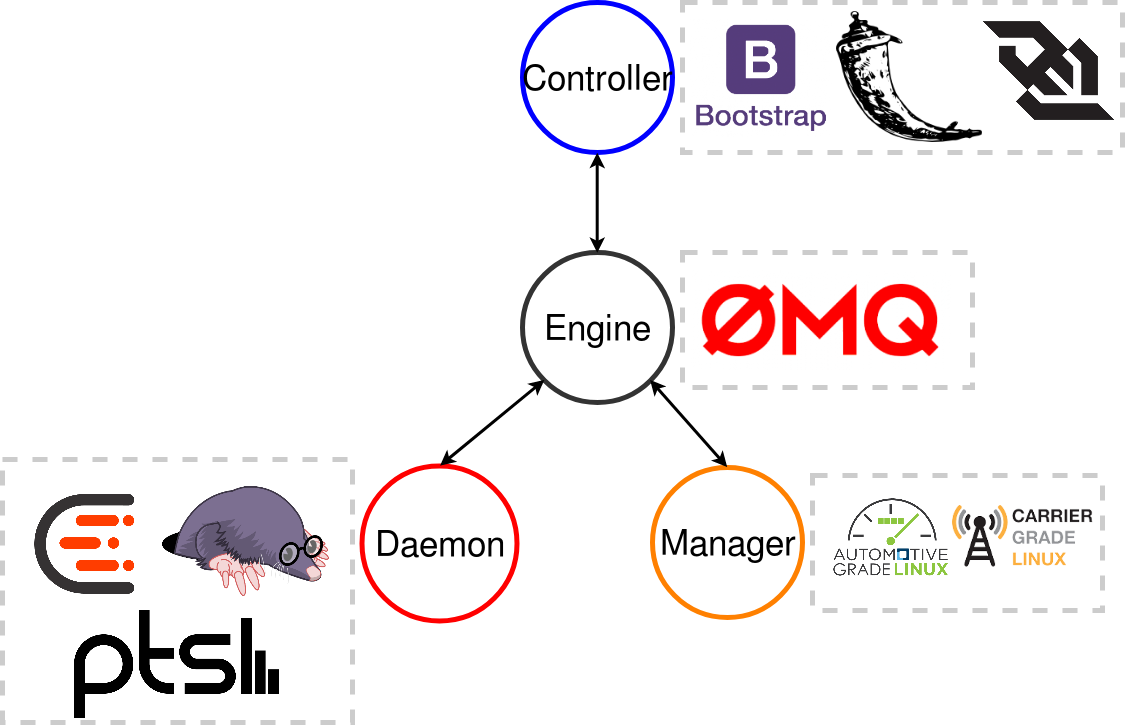
\includegraphics[width=\textwidth]{images/ellida_arch.png}
    \caption{Main components of Ellida framework}
\end{figure}

\subsubsection*{The Engine}
The engine is a central node of communication responsible for coordinating all the other components. It listens for messages and connections and relays them based on the the internal protocol. It is structured around a polling loop inside which specialised functions are called when particular messages arrive. Each function implements a certain part of the internal protocol and usually does as little processing work as possible. The functions only unpack the message, augment it with identification or protocol specific information and then send it to the destination. In the case of Daemon - UI communication the Engine is used to create a direct link between the two. The test results do not pass through the engine, this means that it is not burdened by the heaviest load in the system and the most important part of the communication benefits from less overhead.

The engine is meant to function as a publicly accessible service, ideally paired with an instance of UI, although this is not a requirement. It makes peer discovery easy (Controllers and Daemons) and can abstract away the Daemons, potentially turning the network of connected devices into a uniform resource for parallel testing on multiple targets.

\subsubsection*{The Controller}
Also referred to as the UI, it serves as the main input and output system. Considering that it is implemented as a Flask based web application it also fulfils one of the initial requirements of the project, that test control is available remotely. Although the system is referred as "user interface" it embodies one of the active nodes from the testing network. This means that the backend is just as important as the frontend.

In the current implementation of the communication protocol, one Controller can run tests on only one Daemon at a time. The user can select what part of the specification it intends to test and the information will be bundled together and sent to the target. When a user decides to run a set of tests on a Daemon (target device or VM), the Controller starts listening on a random port and notifies the Engine. The Daemon receives the identification details and creates a direct connection, the connection is only active while the tests run and ends after the Daemon had sent the results back.

\subsubsection*{The Daemon}
The Daemon is the part of the system that triggers the actual testing process. It uses provider modules to execute specific files and to gather the results. As the name suggests, it is intended to run as a daemon process and connects to an Engine instance. Selecting an Engine to connect to is done through a configuration file.

The Daemon is installed through the Yocto build system, in particular, through a Bitbake recipe. The program resides in the system as a globally accessible Python module. While running, the Daemon listens for messages from the Engine, reads the requests and uses a locally available test suite to search for the requested tests. 

\begin{figure}[h!]
  \centering
	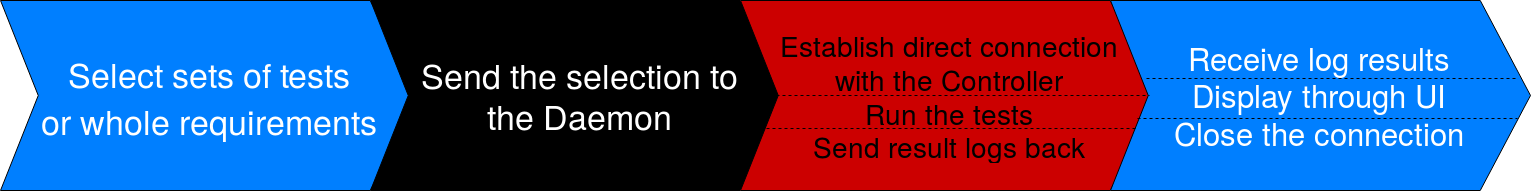
\includegraphics[width=\textwidth]{images/execution_flow2.png}
    \caption{Running a test suite}
\end{figure}

\subsubsection*{The Manager}
One of the more static parts of the framework, the Manager is a collection of parsers and methods for working with files. It can be used to get the latest version of a given specification, parse it and generate the abstract representation - a folder tree containing JSON files. The manager can also check the integrity of the test suite and report standard violations such as creating a test set with more than one provider.

\begin{figure}[h!]
  \centering
	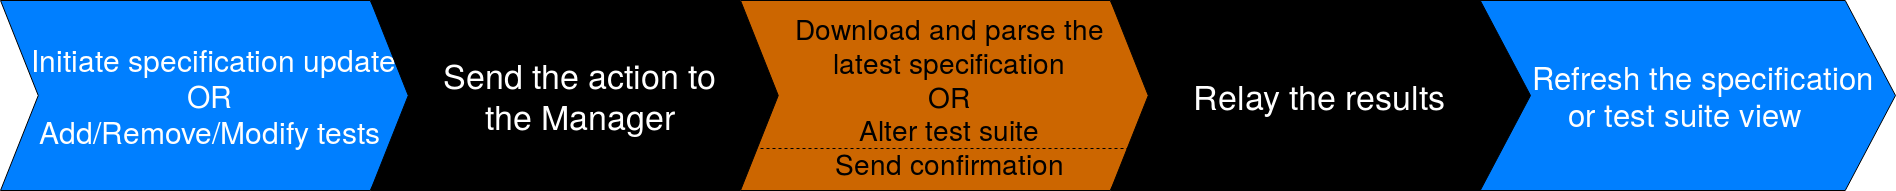
\includegraphics[width=\textwidth]{images/execution_flow1.png}
    \caption{Updating a specification or the test suite}
\end{figure}

\vspace{7mm}

Together, these four components fulfil the requirements of parsing and representing a specification, exposing test controls to the user, manage remote execution of tests, spawn test processes, and return test results.

\section{Yocto integration}

While the core functionality of the Ellida framework can be used on any type of system, for the more advanced features, mainly the providers, the target is expected to be a system generated with Poky. The providers are mostly Linux specific frameworks that require a minimal setup in order do be used. The Ellida framework requires only a Yocto specific setup as it comes embedded inside an OpenEmbedded layer (meta-ellida). The users have to install the layer and its dependencies (meta-oe and meta-python) in their current Yocto setup and run an installation script that appends dependencies to the target Yocto build folder. Bitbake will use the recipes inside the layer to install the Daemon Python project and will also include all the dependencies, mainly, the test providers.

The bitbake recipe contains a description for the standard Python package of the Daemon and setup commands for creating the test suite folder tree. The build system automatically executes the setup.py script and installs the package globally. The recipe for installing the Daemon can be found in the last section - Source code.

